\section{Overview}\label{overview}

\subsection{Abstract}\label{abstract}

\begin{frame}{Abstract}

\begin{itemize}
\itemsep1pt\parskip0pt\parsep0pt
\item
  Describes a pedestrian population trend estimation method using
  location data of smartphone users.
\item
  Intended to be an alternative to traffic censuses using tally
  counters.
\item
  Using smartphone users' location data accumulated on Yahoo! Japan.
\item
  Tackles the problem of data shortage when a target area is a small
  region by using a Gaussian kernel.
\end{itemize}

\end{frame}

\subsection{Background}\label{background}

\begin{frame}{Background}

\begin{itemize}
\itemsep1pt\parskip0pt\parsep0pt
\item
  Knowing the number of pedestrians in a time or place can be an
  essential data source for market research.
\item
  Triditional method: Traffic censuses using tally counters are still
  commonly used.

  \begin{enumerate}
  \def\labelenumi{\arabic{enumi})}
  \itemsep1pt\parskip0pt\parsep0pt
  \item
    Requires many survey crews and much time.
  \item
    Temporal and spatial limitation.
  \end{enumerate}
\item
  Location-based services (LBSs) are widely used by smartphone users
\item
  two problems remain

  \begin{enumerate}
  \def\labelenumi{\arabic{enumi})}
  \itemsep1pt\parskip0pt\parsep0pt
  \item
    How to pick out only pedestrians.
  \item
    How to set the research area and period.
  \end{enumerate}
\end{itemize}

\end{frame}

\section{Data Set}\label{data-set}

\begin{frame}{Data Set}

\begin{itemize}
\itemsep1pt\parskip0pt\parsep0pt
\item
  The location data are provided by smartphone users through services of
  Yahoo! Japan, contains:

  \begin{itemize}
  \itemsep1pt\parskip0pt\parsep0pt
  \item
    Latitude
  \item
    Longitude
  \item
    Horizontal accuracy
  \item
    Time stamp (at a second rate)
  \item
    Anonymized user ID (changes after 24 hours)
  \end{itemize}
\end{itemize}

\end{frame}

\begin{frame}{Data Set}

\begin{figure}
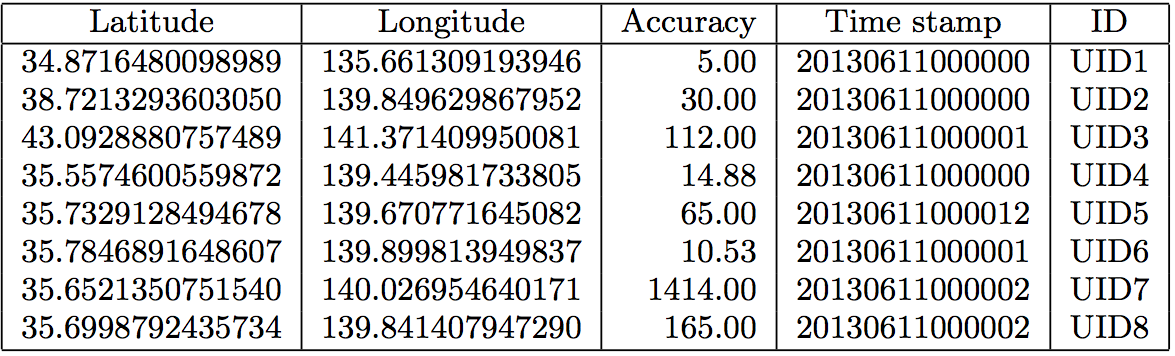
\includegraphics[width = 10cm]{pic1.png}\\
Table: Examples of the location data
\end{figure}

\end{frame}

\begin{frame}{Data Set}

\begin{figure}
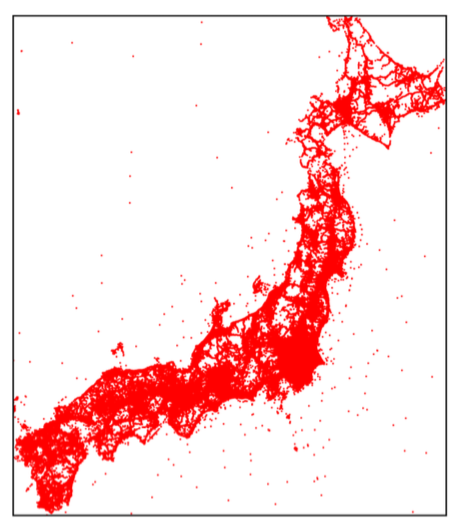
\includegraphics[height = 4cm]{pic2.png}
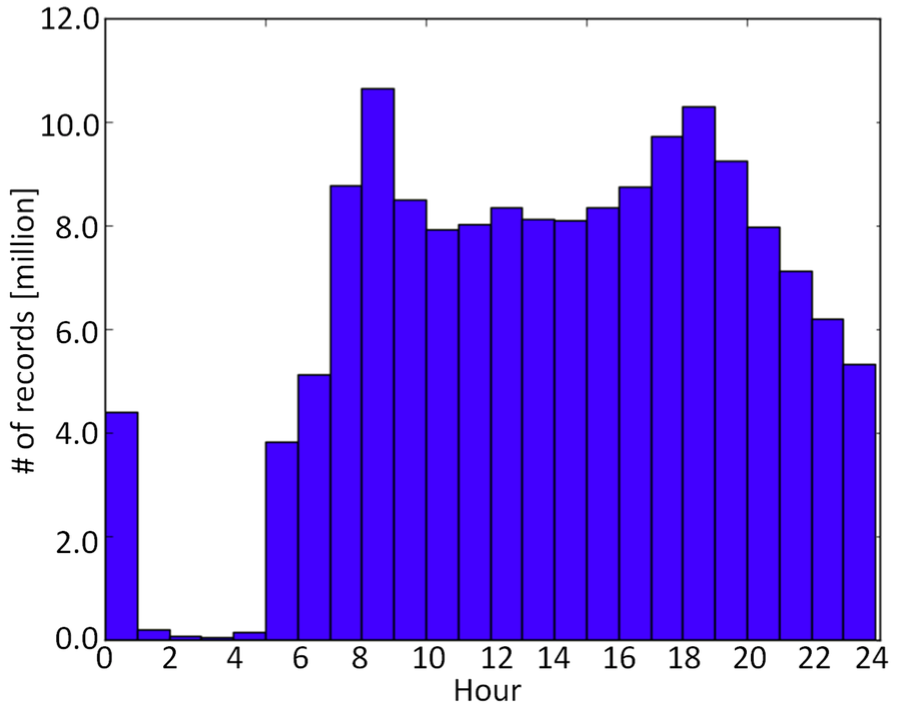
\includegraphics[height = 4cm]{pic3.png}
\end{figure}

\end{frame}

\section{Method}\label{method}

\subsection{Simple approach}\label{simple-approach}

\begin{frame}{A simple approach}

\begin{itemize}
\itemsep1pt\parskip0pt\parsep0pt
\item
  Assumes that the number of records in an area is proportional to the
  people present in the area.

  \begin{itemize}
  \itemsep1pt\parskip0pt\parsep0pt
  \item
    Determine target areas(polygonal) and target days
  \item
    Number of records existing in the area hourly is counted and then
    multiplied by a proper factor.
  \item
    The date has errors more than 300 meters are eliminated.
  \end{itemize}
\end{itemize}

\end{frame}

\begin{frame}{A simple approach}

\begin{figure}
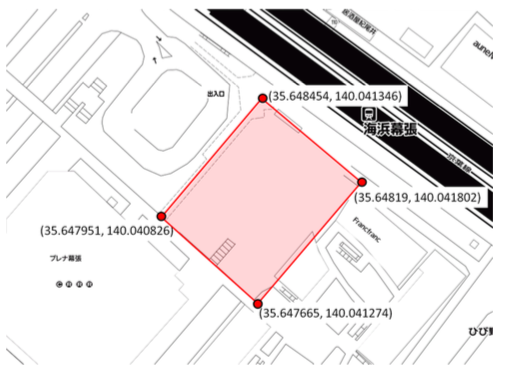
\includegraphics[height = 4cm]{pic4.png}
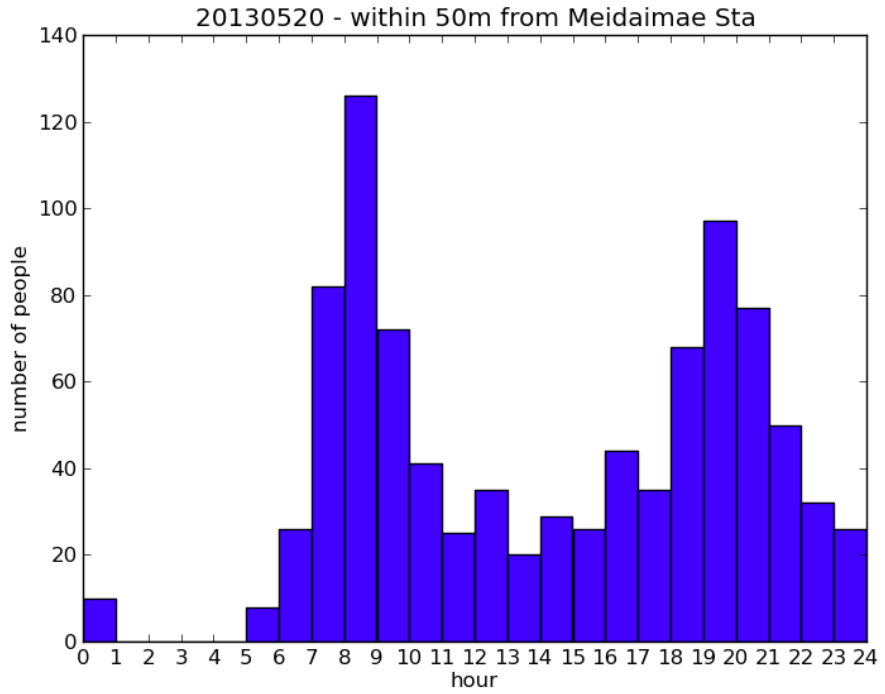
\includegraphics[height = 4cm]{pic5.png}
\end{figure}

\end{frame}

\begin{frame}{Limitation of the simple approach}

\begin{itemize}
\itemsep1pt\parskip0pt\parsep0pt
\item
  Non-pedestrian records

  \begin{itemize}
  \itemsep1pt\parskip0pt\parsep0pt
  \item
    stationary users (e.g.~in offices)
  \item
    passing users (e.g.~on trains)
  \end{itemize}
\item
  Time continuous estimation
\item
  Sparsity with the smallness of target areas.
\end{itemize}

\end{frame}

\subsection{Improvement method}\label{improvement-method}

\begin{frame}{Eliminating non-pedestrian data}

\begin{figure}
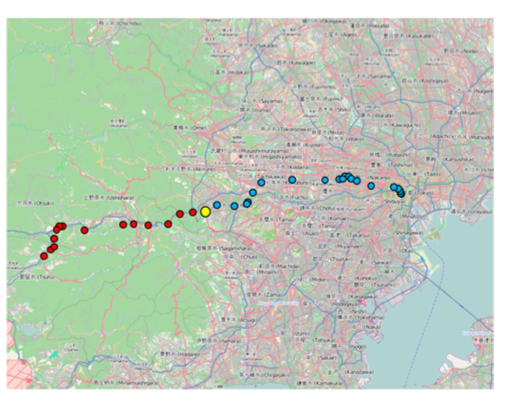
\includegraphics[height = 4cm]{pic6.png} 
\end{figure}

\begin{itemize}
\itemsep1pt\parskip0pt\parsep0pt
\item
  Data are extracted user-by-user(by user id).
\item
  Approximate mean velocity is estimated an hour before or after a
  person visits the target area.
\item
  The records where velocities both before and after are high or near
  zero are eliminated.
\end{itemize}

\end{frame}
